\documentclass[CJK]{beamer}
\usepackage{CJKutf8}
\usepackage{beamerthemesplit}
\usetheme{Malmoe}
\useoutertheme[footline=authortitle]{miniframes}
\usepackage{amsmath}
\usepackage{amssymb}
\usepackage{graphicx}
\usepackage{color}
\usepackage{slashed}
\usepackage{simplewick}
\graphicspath{{../figures/}}
\def\be{\begin{equation}}
\def\ee{\nonumber\end{equation}}
\def\bea{\begin{eqnarray}}
\def\eea{\nonumber\end{eqnarray}}
\def\ii{{\dot{\imath}}}
\def\bch{\begin{CJK}{UTF8}{gbsn}}
\def\ech{\end{CJK}}
\def\bex{\begin{minipage}{0.3\textwidth}
\includegraphics[width=1in]{jugelizi.png}\end{minipage}\begin{minipage}{0.6\textwidth}}
\def\eex{\end{minipage}}
\def\chtitle#1{\frametitle{\bch#1\ech}}
\def\skipline{{\vskip0.1in}}
\def\skiplines{{\vskip0.2in}}
\def\lagr{{\mathcal{L}}}
\def\hamil{{\mathcal{H}}}
\def\vecv{{\mathbf{v}}}
\def\vecx{{\mathbf{x}}}
\def\veck{{\mathbf{k}}}
\def\vecp{{\mathbf{p}}}
\def\vecn{{\mathbf{n}}}
\def\vecA{{\mathbf{A}}}
\def\vecP{{\mathbf{P}}}
\def\vecsigma{{\mathbf{\sigma}}}
\def\hatJn{{\hat{J_\vecn}}}
\def\hatJx{{\hat{J_x}}}
\def\hatJy{{\hat{J_y}}}
\def\hatJz{{\hat{J_z}}}
\def\hatj#1{\hat{J_{#1}}}
\def\hatphi{{\hat{\phi}}}
\def\hatq{{\hat{q}}}
\def\hatpi{{\hat{\pi}}}
\def\vel{\upsilon}
\def\Dint{{\mathcal{D}}}
\def\adag{{\hat{a}^\dagger}}
\def\bdag{{\hat{b}^\dagger}}
\def\cdag{{\hat{c}^\dagger}}
\def\ddag{{\hat{d}^\dagger}}
\def\hata{{\hat{a}}}
\def\hatb{{\hat{b}}}
\def\hatc{{\hat{c}}}
\def\hatd{{\hat{d}}}
\def\hatN{{\hat{N}}}
\def\hatH{{\hat{H}}}
\def\hatp{{\hat{p}}}
\def\Fup{{F^{\mu\nu}}}
\def\Fdown{{F_{\mu\nu}}}
\def\newl{\nonumber \\}
\def\SIkm{\mathrm{km}}
\def\SIyr{\mathrm{yr}}
\def\SIGyr{\mathrm{Gyr}}
\def\SIeV{\mathrm{eV}}
\def\SIGeV{\mathrm{GeV}}
\def\SIm{\mathrm{m}}
\def\SIcm{\mathrm{cm}}
\def\SIJ{\mathrm{J}}
\def\SIs{\mathrm{s}}
\def\SIkg{\mathrm{kg}}
\def\SIg{\mathrm{g}}
\def\vece{\mathrm{e}}
\def\bmat#1{\left(\begin{array}{#1}}
\def\emat{\end{array}\right)}
\def\bcase#1{\left\{\begin{array}{#1}}
\def\ecase{\end{array}\right.}
\def\calM{{\mathcal{M}}}
\def\calT{{\mathcal{T}}}
\def\calR{{\mathcal{R}}}
\def\barpsi{\bar{\psi}}
\def\baru{\bar{u}}
\def\barv{\bar{\upsilon}}
\def\bmini#1{\begin{minipage}{#1\textwidth}}
\def\emini{\end{minipage}}
\def\qeq{\stackrel{?}{=}}
\def\torder#1{\mathcal{T}\left(#1\right)}
\def\rorder#1{\mathcal{R}\left(#1\right)}


\title{Quantum Field Theory I \\ Openmind Homework}
  \author{}
  \date{}


\begin{document}

\begin{frame}
 
\begin{center}
\begin{Large}
\bch
量子场论 I 

{\vskip 0.3in}

脑洞大开作业 (10分,共5题每题2分,每题如有特别精彩巧妙的解法额外加1分bonus分, 但bonus分仅在期末总分不超过100分的情况下有效)

\skipline
允许搜索查阅讨论请教。允许使用任何文献(包括讲义)中的结论,但请指出出处。

\skipline
交作业时间: 期末考试前任何时间

\ech
\end{Large}
\end{center}

\vskip 0.2in

\bch
课件下载
\ech
https://github.com/zqhuang/SYSU\_QFTI

\end{frame}


\begin{frame}
\chtitle{第1题 二维空间的Casimir力(2分)}
\bch
假设“脑洞大开世界”是2维空间加1维时间的平直时空,时空度量元为
$$ds^2 = (dx^0)^2 - (dx^1)^2-(dx^2)^2$$
在这个世界里的“脑洞大开人”发现真空中的相距为$d$的很长的(长度$\gg d$)两根平行金属线之间有大小为$F$的相互作用力,他们认为这是两条金属线之间的真空能的改变引起的作用力,并把这种力称为Casimir力。现在问,当把金属线之间的距离变为$d/2$,Casimir力变为多大?

\ech
\end{frame}

\begin{frame}
\chtitle{第2题 只有两个自由度的“量子场”(2分)}
\bch
\begin{minipage}{0.3\textwidth}
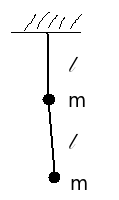
\includegraphics[width=1.in]{shuangbai.png}
\end{minipage}
\begin{minipage}{0.5\textwidth}
如图,在一个长度为$\ell$,质量为$m$的理想刚性单摆下再悬挂一个相同的单摆。节点处都认为可以无阻力自由在所示的平面内转动。本地重力常数为$g$。试求该系统的量子零点能。

\end{minipage}
\ech
\end{frame}

\begin{frame}
\chtitle{第3题 奇怪的一维量子场。(2分)}
\bch
\begin{minipage}{0.3\textwidth}
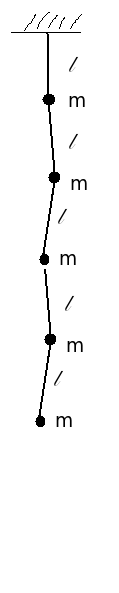
\includegraphics[width=0.5in]{duobai.png}
\end{minipage}
\begin{minipage}{0.5\textwidth}
把上题推广到$N$个长度为$\ell$,质量为$m$的理想刚性单摆首位连接挂起来(如左图给出了一个$N=5$的例子),所有的单摆都可以无摩擦在所示的平面内转动。记系统的总量子零点能为$E_N$。当$N\rightarrow \infty$时,$E_N/N^{3/2}$趋向于一个常数,试计算这个常数(用$\ell$, $g$, $m$来表示)。

\skipline
{\scriptsize 
注:精确解的求解需要比较巧妙的手段。如果你找不到求解精确解的办法,请尽你所能地估算一个范围。
}
\end{minipage}

\ech
\end{frame}




\begin{frame}
\chtitle{第4题 环上的量子场(2分)}
\bch
假设“脑洞大开世界”为一个一维圆环加上一维时间,时空度量元为
$$ds^2 = dt^2 - R^2 d\theta^2$$
其中$R>0$为固定常数,$(t,\theta)$为时空坐标。在这个时空里的质量为$m$的实标量场$\phi(t,\theta)$满足周期性边界条件
$$\phi(t,\theta+2\pi) = \phi(t,\theta)$$
其自由场拉氏量为
$$L_{\rm free} = \int_0^{2\pi}d\theta\ \frac{1}{2}\left[\left(\frac{\partial\phi}{\partial t}\right)^2-\frac{1}{R^2}\left(\frac{\partial\phi}{\partial\theta}\right)^2-m^2\phi^2\right]$$
试把$\phi$场量子化。

\ech
\end{frame}


\begin{frame}
\chtitle{第5题 环上的量子场的散射(2分)}
\bch
给上题中的场$\phi$加一个自相互作用的拉氏量,
$$L = L_{\mathrm{free}} - \int_0^{2\pi}d\theta\ \frac{\lambda}{4!}\phi^4$$
其中$\lambda\ll 1$为耦合常数。

试证明,这个场的两个粒子不可能发生散射变成和初态不同的两个粒子。

\ech
\end{frame}


\end{document}
